%\documentclass[fleqn]{report}
%\usepackage{graphicx} % om PostScript plaatje in te lassen
%\usepackage{here}     % voor geforceerde plaatsing figuren
%\usepackage{amsmath}
%\textwidth=17.0cm
%\textheight=22.0cm
%\topmargin=-1cm
%\oddsidemargin=-0.3cm
%\evensidemargin=-0.3cm
%
%%packages
%\usepackage{amsmath}
%\usepackage{cite}
%\usepackage[toc,page]{appendix}
%\usepackage{fancyvrb}
%\usepackage{tikz}
%\usepackage{multicol}
%\usepackage{framed}
%\usepackage{pgfplots}
%\usepackage{fixltx2e}
%\usepackage{subfigure}
%\usepackage{lscape}
%\usepackage{enumitem}
%\usepackage{filecontents}
%
%%tikz labraries
%\usetikzlibrary{matrix}
%\usetikzlibrary{decorations.pathreplacing}
%\usetikzlibrary{positioning}
%\usetikzlibrary{calc}
%\usetikzlibrary{shapes,arrows, chains}
%\usetikzlibrary{intersections}
%\usetikzlibrary{decorations.markings}
%\usetikzlibrary{calc,intersections}
% \usetikzlibrary{svg.path}
% \usetikzlibrary{patterns}
%\usepackage{xcolor}
%%\usetikzlibrary{decorations.pathreplacing,bending}
%
%%extra instellingen
%\newlist{aims}{enumerate}{1}
%\setlist[aims,1]{
%  label={*},
%  leftmargin=*,
%  align=left,
%  labelsep=2mm,
%}
%
%\newlist{aims2}{enumerate}{1}
%\setlist[aims2,1]{
%  label={},
%  leftmargin=0pt,
%  align=left,
%  labelsep=4mm,
%}
%
%\newlist{aims3}{enumerate}{1}
%\setlist[aims3,1]{
%  label={-},
%  leftmargin=2cm,
%  align=left,
%  labelsep=0.4mm,
%}
%
%\usepackage{pgfplots}
%
%\begin{document}


\begin{tikzpicture}
\footnotesize

% used shapes
\tikzstyle{block} = [rectangle, draw, node distance = 0.5cm, text width=4cm, text centered, minimum height=1cm]
\tikzstyle{diamond_thing} = [diamond, draw, node distance = 0.5cm, text centered, minimum height=1cm]
\tikzstyle{blokje} = [rectangle, draw, rounded corners = 5pt, node distance = 0.5cm, text width=2cm, text centered, minimum height=0.5cm,fill=purple!20]
\tikzstyle{blockrounded} = [rectangle, draw, rounded corners = 5pt, node distance = 1cm, fill=yellow!20, text width=3cm, text centered, minimum height=0.5cm]
\tikzstyle{blockroundedred} = [rectangle, draw, rounded corners = 5pt, node distance = 1cm, fill=red!20, text width=3cm, text centered, minimum height=0.5cm]


% design situation
\node [block] (design_situation) {Design situation};
 
% iputs of the design situation
\node [blockrounded, left = of design_situation, align=center, anchor=east]  (referencelocation) {Location of structure};
\node [blockrounded, above left =of design_situation, align=center, anchor=south]  (location_on_building) {Orientation of structure};
\node [blockrounded, above right = of design_situation, align=center,anchor=south]  (referencearea) {Terrain parameters};
\node [blockrounded, right = of design_situation, align=center,anchor=west]  (orientation) {Size fa\c{c}ade element};
\node [blockrounded, above left = 2.3cm and -0.4 cm of design_situation, align=center, anchor=south]  (terrain_roughness) {Location of fa\c{c}ade element};
\node [blockrounded, above right = 2.3cm and -0.4cm of design_situation, align=center, anchor=south]  (wind_directions) {Type of material \\ fa\c{c}ade element};
\node [blockrounded, below left = of design_situation, align=center, anchor=east]  (material_type) {Consequence Class \\ and lifetime \\ of structure};
\node [blockrounded, below right = of design_situation, align=center, anchor=west]  (required_reliability) {Incident wind directions \\ $\theta_i$ for $i=1,...k$};


% lines of inputs of the design situation
\draw  (referencelocation) -- (design_situation);
\draw (location_on_building) -- (design_situation);	
\draw  (referencearea)-- (design_situation);	
\draw  (orientation) -- (design_situation);	
%\draw  (beta_required) -- (design_situation);	
\draw  (terrain_roughness) -- (design_situation);
\draw  (wind_directions) -- (design_situation);
\draw  (material_type) -- (design_situation);
\draw  (required_reliability) -- (design_situation);

% incident wind direction
\node [block, below = of design_situation.south] (initialize_wind_direction) {Initialize \\ $i=1$};
\node [diamond_thing, below = of initialize_wind_direction.south,align=center] (condition_wind_direction) {Condition \\ $i\stackrel{?}{\leq} k$};
\draw [-triangle 45] (design_situation) -- (initialize_wind_direction) ;
\draw [-triangle 45] (initialize_wind_direction.south) -- (condition_wind_direction) ;


% RESISTANCE PART
\node [block, below left = 3cm and -0.2cm of condition_wind_direction,anchor=east] (stochastic_strength) {Structural resistance $R$ \\ 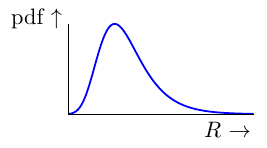
\includegraphics[height=2cm]{tikz/images/PDF_resistance}}   ;

% LOAD PART 
\node [block, below right = 3cm and -0.2cm of condition_wind_direction,anchor=west] (stochastic_load) {Wind load $S(\theta_i)$ \\ 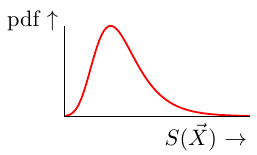
\includegraphics[height=2cm]{tikz/images/PDF_load}}   ;

% LINES TOWARDS LOAD AND STRENGTH
\draw (condition_wind_direction.south)  -- +(0,-0.5) node [above right] (TextNode) {TRUE} ;
\draw [-triangle 45] (condition_wind_direction.south)+(0,-0.5) -| (stochastic_strength); % strength
\draw [-triangle 45] (condition_wind_direction.south)+(0,-0.5) -| (stochastic_load); % load

% LIMIT STATE
\node [block, below = 5 cm of condition_wind_direction.south, anchor=north] (limit_state_function) {Limit state function\\ $Z(\theta_i) = R - S(\theta_i)$ };

\node [block, below =of limit_state_function, anchor=north] (conditional)  {Conditional failure probability \\ $P_{f}(\theta_i)|\theta_i$};

\node [block, below =of conditional, anchor=north] (unconditional)  {Unconditional failure probability\\ $P_{f}(\theta_i)=P_{f}(\theta_i)|\theta_i \cdot P(\theta_i)$};

\node [block, below =of unconditional, anchor=north] (next)  {Next \\ $i=i+1$};




% LINES TO UNCONDITIONAL FAILURE PROBAIBLITY
\draw (stochastic_strength.south) |- (0,-9.5);
\draw (stochastic_load.south) |- (0,-9.5);
\draw [-triangle 45] (0,-9.5)-- (limit_state_function);
\draw [-triangle 45](limit_state_function) -- (conditional);
\draw [-triangle 45] (conditional) -- (unconditional);
\draw [-triangle 45] (unconditional) -- (next);
\draw (next.east) -- +(3,0);
\draw [-triangle 45](next.east)+(3,0) |- (condition_wind_direction);


% IF ALL DIRECTIONS ARE DONE
\node [block, left = 5cm of condition_wind_direction, anchor=east] (total)  {Total failure probability\\ $P_{f,total}=\sum_{i=1}^k P_{f}(\theta_i) $};
\node [block, below =of total, anchor=north] (reliability)  {Reliability index \\ $\beta_{total} = -\Phi_u^{-1}(P_{f,total})$};

% LINES FOR ALL DIRECTIONS
\draw [-triangle 45] (condition_wind_direction.west) -- (total.east) node [midway, above] (TextNode) {FALSE} ;
\draw [-triangle 45] (total.south) -- (reliability.north);





\end{tikzpicture}




%
%%
%\end{document}